\renewcommand{\FileName}{agree}
% slide template
\begin{frame}
  \frametitle{Observer Agreement}
  \begin{itemize}
	\item {\large\bfseries Inter-observer agreement} often used as to assess 
reliability of a subjective classification or assessment procedure
      \begin{itemize*}
        \item $\rightarrow$ square table, Rater 1 x Rater 2
	    \item Levels: diagnostic categories (normal, mildly impaired, severely
		impaired)
	  \end{itemize*}
	\item{\large\bfseries Agreement vs.\ Association:} Ratings can be strongly associated 
	without strong agreement
	\item{\large\bfseries Marginal homogeneity:}  Different frequencies of
	category use by raters affects measures of agreement
	\item{\large\bfseries Measures of Agreement:}
      \begin{itemize*}
	  \item Intraclass correlation:  ANOVA framework--- multiple raters!
	  \item Cohen's $\kappa$: compares the observed agreement, \(P_o  =
\sum p_{ii}\), to agreement expected by chance if the two observer's
ratings were independent, \(P_c = \sum p_{i+} \,  p_{+i}\).
  \begin{equation*} \label{eq:kappa}
  \kappa =  \frac{ P_o - P_c } { 1 - P_c }
  \end{equation*}
      \end{itemize*}
  \end{itemize}
\end{frame}

\subsection[Cohen's kappa]{Cohen's kappa}
\begin{frame}[fragile]
  \frametitle{Cohen's $\kappa$}
  \begin{itemize*}
      \item Properties of Cohen's $\kappa$:
    	\begin{itemize*}
		\item perfect agreement: \(\kappa = 1\)
		\item minimum \(\kappa\) may be \(< 0\); lower bound depends on marginal
       totals
	    \item Unweighted $\kappa$: counts only diagonal cells (same
       category assigned by both observers).
	    \item Weighted $\kappa$: allows partial credit for near agreement.
		(Makes sense only when the categories are \emph{ordered}.)
		\end{itemize*}
	  \item Weights:  
    	\begin{itemize*}
			\item Cicchetti-Alison (inverse integer spacing) vs.\
	  		\item Fleiss-Cohen (inverse square spacing)
 		\end{itemize*}
 \end{itemize*}

\begin{Output}[fontsize=\footnotesize]
       Integer Weights                 Fleiss-Cohen Weights
   1     2/3     1/3       0          1     8/9     5/9      0
 2/3       1     2/3     1/3        8/9       1     8/9    5/9
 1/3     2/3       1     2/3        5/9     8/9       1    8/9
   0     1/3     2/3       1          0     5/9     8/9      1
\end{Output}

\end{frame}

\begin{frame}[fragile]
  \frametitle{Cohen's $\kappa$: Example}
The table below summarizes responses of 91
married couples to a questionnaire item,

\begin{quote}
Sex is fun for me and my partner (a) Never or occasionally, (b)
fairly often, (c) very often, (d) almost always.  
\end{quote}
\vspace{2em}

\begin{Output}
              --------- Wife's Rating --------
Husband's     Never   Fairly     Very   Almost
Rating          fun    often    Often   always    |   SUM    
--------------------------------------------------+-------
Never fun         \sasemph{7}        7        2        3    |    19
Fairly often      2        \sasemph{8}        3        7    |    20
Very often        1        5        \sasemph{4}        9    |    19
Almost always     2        8        9       \sasemph{14}    |    33
--------------------------------------------------+-------
SUM              12       28       18       33    |    91    
\end{Output}
\end{frame}

\begin{frame}[fragile]
  \frametitle{Computing $\kappa$ with SAS}
  \begin{itemize}
	\item \PROC{FREQ}: Use \texttt{AGREE} option on \texttt{TABLES} statement
      \begin{itemize*}
	  \item Gives both unweighted and weighted $\kappa$ (default: CA weights)
	  \item \texttt{AGREE (wt=FC)} uses Fleiss-Cohen weights
	  \item Bowker's \citep{Bowker:48} test of symmetry: $H_0 : p_{ij} = p_{ji}$
	  \end{itemize*}
  \end{itemize}

\vspace{2ex}
\begin{Input}[fontsize=\footnotesize,label=\fbox{\texttt{kappa3.sas}},baselinestretch=0.8]
title 'Kappa for Agreement';
data fun;
   do Husband = 1 to 4;
   do Wife    = 1 to 4;
      input count @@;
      output;
      end; end;
datalines;
 7     7     2      3
 2     8     3      7
 1     5     4      9
 2     8     9     14
;
proc freq;
  weight count;
  tables Husband * Wife / noprint \sasemph{agree};      \sascomment{/* default: CA weights*/}
  tables Husband * Wife / noprint \sasemph{agree(wt=FC)};
\end{Input}
\end{frame}

\begin{frame}[fragile]
  \frametitle{Computing $\kappa$ with SAS}
Output (CA weights):
\begin{Output}[baselinestretch=0.8,gobble=3]
              Statistics for Table of Husband by Wife

                         Test of Symmetry
                      -----------------------
                      Statistic (S)    3.8778
                      DF                    6
                      Pr > S           0.6932

                          Kappa Statistics
 
    Statistic          Value       ASE     95% Confidence Limits
    ------------------------------------------------------------
    Simple Kappa      0.1293    0.0686      -0.0051       0.2638
    Weighted Kappa    0.2374    0.0783       0.0839       0.3909

                          Sample Size = 91
\end{Output}
Using Fleiss-Cohen weights:
\begin{Output}[gobble=3]
    Weighted Kappa    0.3320    0.0973       0.1413       0.5227
\end{Output}
\end{frame}

\begin{frame}[fragile]
  \frametitle{Observer agreement: Multiple strata}
  \begin{itemize}
	\item When the individuals rated fall into multiple groups, one can test for:
      \begin{itemize*}
	  \item Agreement within each group
	  \item Overall agreement (controlling for group)
	  \item Homogeneity: Equal agreement across groups
      \end{itemize*}
  \end{itemize}
Example: Diagnostic classification of mulitiple sclerosis by two neurologists,
for two populations \citep{LandisKoch:77}
\begin{listing}[baselinestretch=0.8]
                 Winnipeg patients        New Orleans patients
  NO rater:
                Cert Prob  Pos Doubt      Cert Prob  Pos Doubt 
                --------------------      --------------------
Winnipeg rater:
 Certain MS      38    5    0    1          5    3    0    0
 Probable        33   11    3    0          3   11    4    0
 Possible        10   14    5    6          2   13    3    4
 Doubtful MS      3    7    3   10          1    2    4   14 
\end{listing}
Analysis:
\begin{Input}[numbers=none]
 proc freq;
   tables \sasemph{strata} * rater1 * rater2 / \sasemph{agree};
\end{Input}

\end{frame}

\begin{frame}[fragile]
  \frametitle{Observer agreement: Multiple strata}
\begin{Input}[fontsize=\footnotesize,label=\fbox{\texttt{msdiag.sas}},baselinestretch=0.8]
data msdiag;
  do patients='Winnipeg  ', 'New Orleans';
     do N_rating = 1 to 4;
        do W_rating = 1 to 4;
           input count @;
           output;
           end;
        end;
     end;
 label N_rating = 'New Orleans neurologist'
       W_rating = 'Winnipeg neurologist';
datalines;
38  5  0  1
33 11  3  0
10 14  5  6
 3  7  3 10
 5  3  0  0
 3 11  4  0
 2 13  3  4
 1  2  4 14
;

*-- Agreement, separately, and controlling for Patients;
proc freq data=msdiag;
   weight count;
   tables \sasemph{patients} * N_rating * W_rating / norow nocol nopct agree;
\end{Input}
\end{frame}

\begin{frame}[fragile]
  \frametitle{Observer agreement: Multiple strata}
Output, strata 1: (New Orleans patients):
\begin{Output}[baselinestretch=0.8,gobble=3]
           Statistics for Table 1 of N_rating by W_rating
                Controlling for patients=New Orleans

                         Test of Symmetry
                      -----------------------
                      Statistic (S)    9.7647
                      DF                    6
                      Pr > S           0.1349

                          Kappa Statistics
 
    Statistic          Value       ASE     95% Confidence Limits
    ------------------------------------------------------------
    Simple Kappa      0.2965    0.0785       0.1427       0.4504
    Weighted Kappa    0.4773    0.0730       0.3341       0.6204

                          Sample Size = 69
\end{Output}
\end{frame}

\begin{frame}[fragile]
  \frametitle{Observer agreement: Multiple strata}

Output, strata 2: (Winnipeg patients):
\begin{Output}[baselinestretch=0.8,gobble=3]
           Statistics for Table 2 of N_rating by W_rating
                 Controlling for patients=Winnipeg

                          Test of Symmetry
                      ------------------------
                      Statistic (S)    46.7492
                      DF                     6
                      Pr > S            <.0001

                          Kappa Statistics
 
    Statistic          Value       ASE     95\% Confidence Limits
    ------------------------------------------------------------
    Simple Kappa      0.2079    0.0505       0.1091       0.3068
    Weighted Kappa    0.3797    0.0517       0.2785       0.4810

                         Sample Size = 149
\end{Output}
\end{frame}

\begin{frame}[fragile]
  \frametitle{Observer agreement: Multiple strata}

Overall test:
\begin{Output}[baselinestretch=0.8,gobble=3]
            Summary Statistics for N_rating by W_rating
                      \sasemph{Controlling for patients}

                     Overall Kappa Coefficients
 
    Statistic          Value       ASE     95\% Confidence Limits
    ------------------------------------------------------------
    Simple Kappa      0.2338    0.0424       0.1506       0.3170
    Weighted Kappa    0.4123    0.0422       0.3296       0.4949
\end{Output}
Homogeneity test:  $H_0: \kappa_1 = \kappa_2 = \dots = \kappa_k$
\begin{Output}[baselinestretch=0.8]
                \sasemph{Tests for Equal Kappa Coefficients}
 
          Statistic         Chi-Square    DF    Pr > ChiSq
          ------------------------------------------------
          Simple Kappa          0.9009     1      0.3425  
          Weighted Kappa        1.1889     1      0.2756  

                      Total Sample Size = 218
\end{Output}
\end{frame}

\begin{frame}
 \frametitle{Observer agreement: SAS 9.3 ODS graphs}
% three figures in tabular layout
 \begin{minipage}[c]{.5\linewidth}
  \centering
  \includegraphics[width=.95\linewidth]{fig/msdiag-WtKappaPlot}
    \\ \texttt{agree} option $\rightarrow$ plots of CIs for $\kappa$ ... 
 \end{minipage}%
 \begin{minipage}[c]{.5\linewidth}
  \centering
  \begin{tabular}{c}
  \includegraphics[width=.8\linewidth]{fig/msdiag-AgreePlot1} \\
  \includegraphics[width=.8\linewidth]{fig/msdiag-AgreePlot2} \\
   ... and agreement plots (next)
  \end{tabular}
 \end{minipage}
\end{frame}



\subsection{Observer Agreement Chart}
\begin{frame}
  \frametitle{Bangdiwala's Observer Agreement Chart}
  \begin{itemize}
	\item The observer agreement chart \cite{Bangdiwala:87} provides
      \begin{itemize*}
	  \item a simple graphic representation of the strength of agreement, and 
 	  \item a measure of strength of agreement with an intuitive
interpretation.
	  \end{itemize*}
	 

	\item Construction: 
      \begin{itemize*}
	  \item \(n \times  n\) square, $n$=total sample size
	  \item Black squares, each of size \(n_{ii} \times  n_{ii} \rightarrow\)  observed agreement
	  \item Positioned within larger rectangles, each of size \(n_{i+} \times  n_{+i} \rightarrow\) maximum possible agreement
	  \item $\Rightarrow$ visual impression of the strength of agreement is
	  \end{itemize*}
  \begin{equation*}
  B_N  =
  \frac{ \mbox{area of dark squares}}
  { \mbox{area of rectangles}}  =
  \frac{ \sum_i^k \,  n_{ii}^2 }
  { \sum_i^k \,  n_{i+} \,  n_{+i} }
  \end{equation*}
  \end{itemize}
\end{frame}

\begin{frame}
Husbands and wives: $B_N = .146$
 \begin{center}
 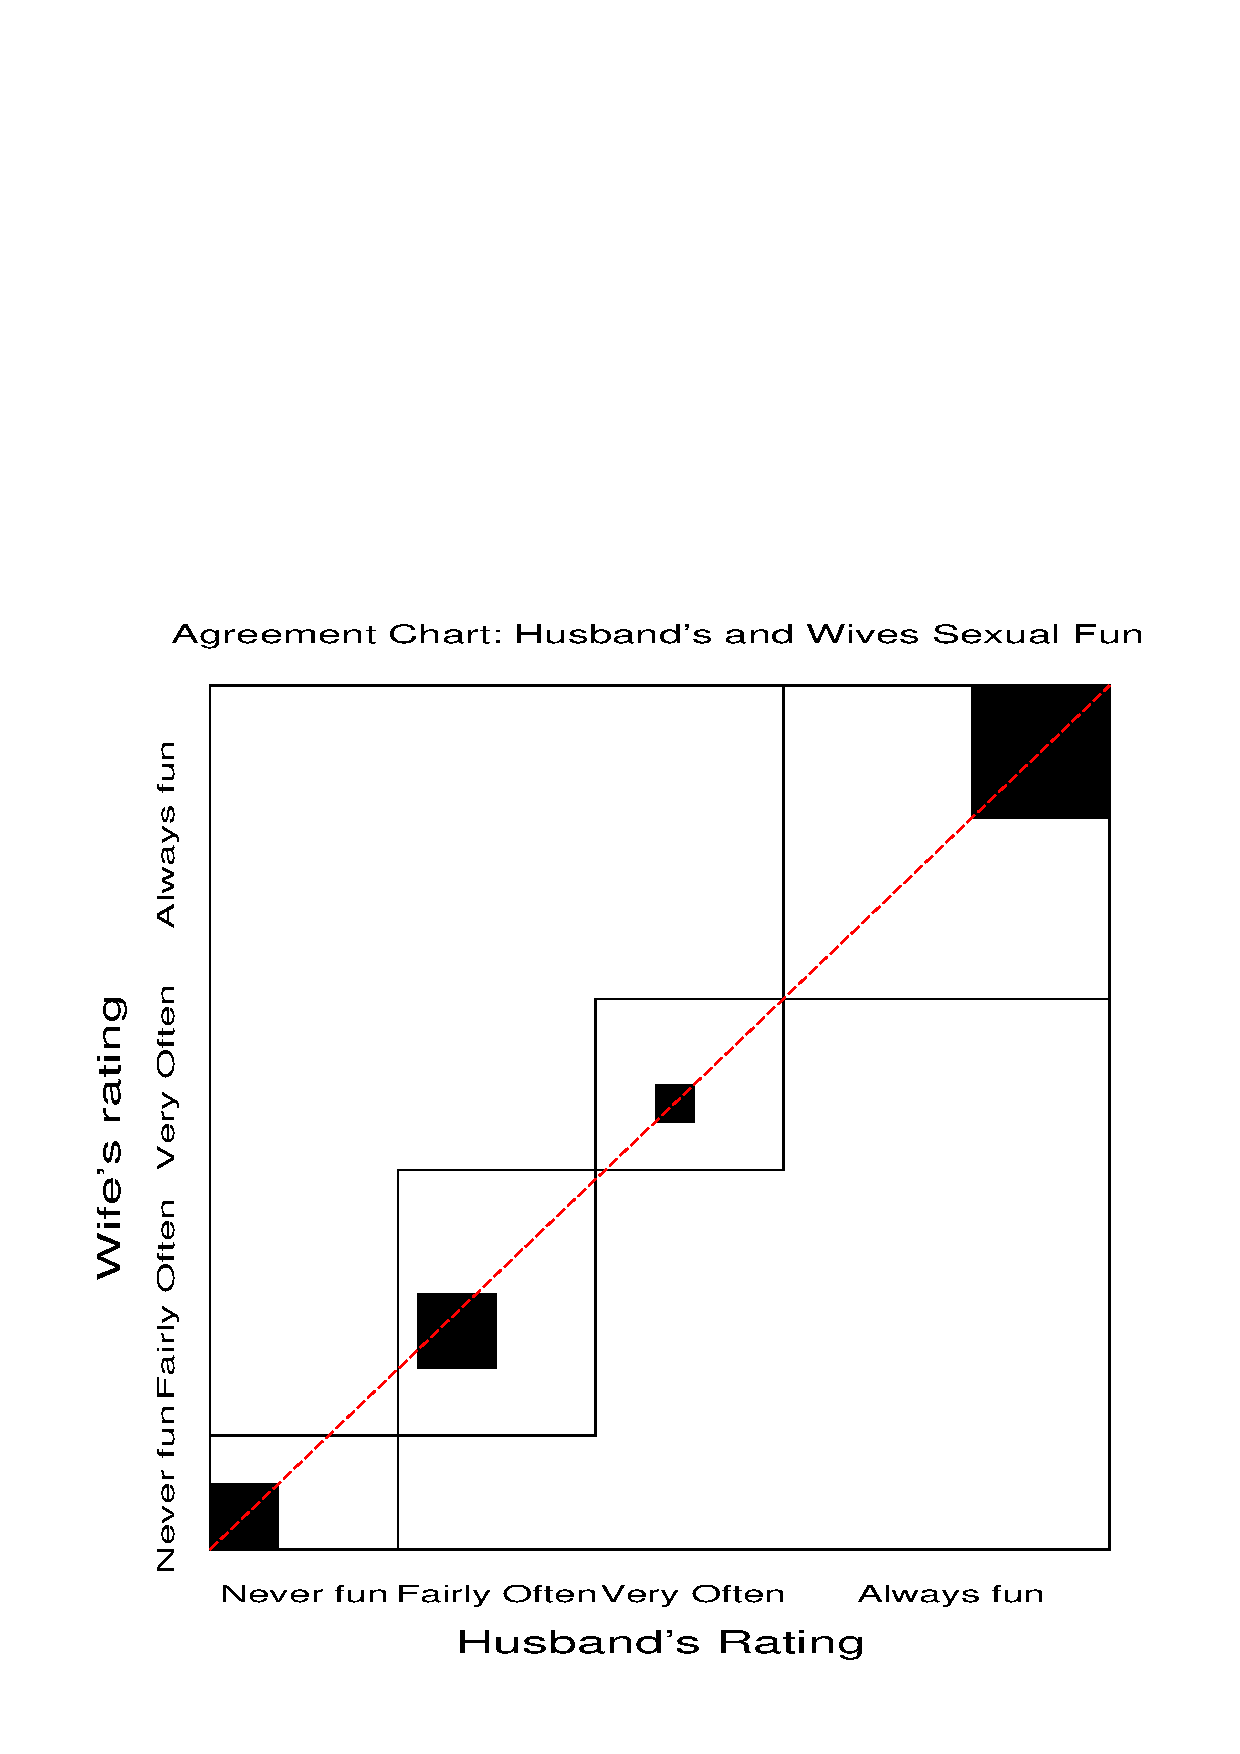
\includegraphics[width=.7\textwidth,clip,keepaspectratio]{fig/agreemt1}
 \end{center}
  
\end{frame}

\begin{frame}
  \frametitle{Weighted Agreement Chart: Partial agreement}
 Partial agreement:
include  weighted contribution from off-diagonal cells, \(b\)
steps from the main diagonal, using weights $ 1 > w_1 > w_2 > \cdots$.

  \[
 \left.
 \begin{array}{ccccc}
   &  & n_{i-b,i} &  & \\
    &  & \vdots    &  & \\
    n_{i, i-b} & \cdots & n_{i, i} & \cdots & n_{i, i+b} \\
    &  & \vdots    &  & \\
   &  & n_{i-b,i} &  &
 \end{array}
  \right.
  \qquad
 \left.
 \begin{array}{ccccc}
   &  & w_2 &  & \\
   &  & w_1 &  & \\
 w_2 & w_1 & 1 & w_1 & w_2 \\
   &  & w_1 &  & \\
   &  & w_2 &  & \\
 \end{array}
  \right.
  \]

  \begin{itemize}
	\item Add shaded rectangles, size $\sim$ sum of frequencies, \(A_{bi}\), within $b$ steps of main diagonal
	\item $\Rightarrow$ weighted measure of agreement,
  \[
  B_N^w  =
  \frac{ \mbox{weighted sum  of agreement}}
  { \mbox{area of rectangles} }  =
  1 - \frac{ \sum_i^k \,
  [ n_{i+} n_{+i} - n_{ii}^2  -
  \sum_{b=1}^q \,  w_b  A_{bi} ] }
  { \sum_i^k \,  n_{i+} \,  n_{+i} }
  \]
  \end{itemize}
\end{frame}

\begin{frame}
Husbands and wives: $B_N^w = .628$ with $w_1 = 8/9$
 \begin{center}
 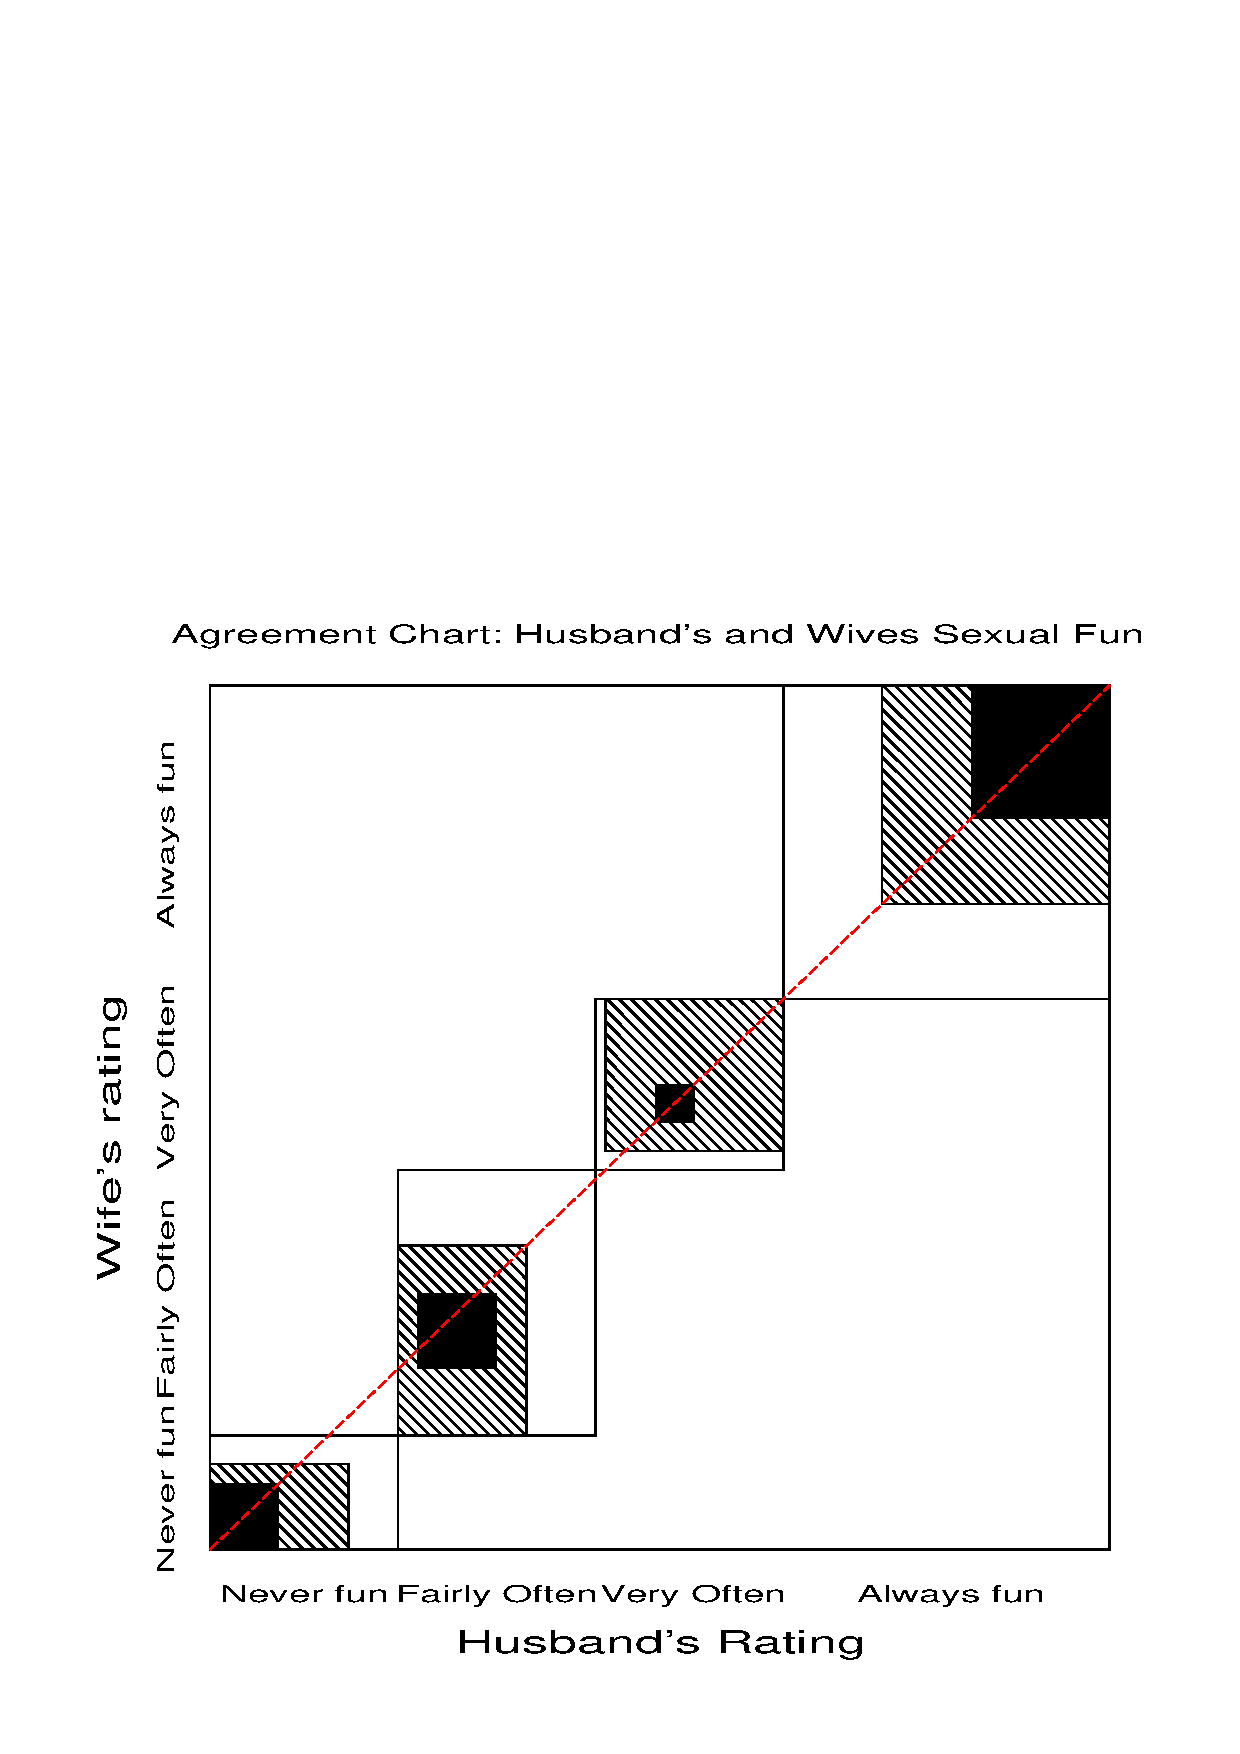
\includegraphics[width=.7\textwidth,clip,keepaspectratio]{fig/agreemt2}
 \end{center}
\end{frame}

\renewcommand{\FileName}{agree-Sex-SAS}
\begin{frame}[fragile]
\frametitle{\macrot{agreeplot}}
\begin{Input}[gobble=1,baselinestretch=0.8,fontsize=\footnotesize]
 proc format;
  value \sasemph{rating} 1='Never_fun' 2='Fairly_often' 
               3='Very_often' 4='Almost_always';
 data sexfun;
   \sasemph{format Husband Wife rating.;}
   do Husband = 1 to 4;
   do Wife    = 1 to 4;
     input count @@;
     output;
     end; end;
 datalines;
  7     7     2      3
  2     8     3      7
  1     5     4      9
  2     8     9     14
 ;

 \sascomment{*-- Convert numbers to formatted values;}
 %table(data=sexfun, var=Husband Wife, char=true, weight=count, out=table);
 %agreeplot(data=table, var=Husband Wife, title=Husband and Wife Sexual Fun);
\end{Input}
\begin{itemize*}
 \item To preserve ordering, integer values are used for Husband and Wife
 \item A SAS format is used to provide value labels
 \item The \macro{table} converts numeric $\rightarrow$ character
\end{itemize*}

\end{frame}
\renewcommand{\FileName}{agree-Sex-R}
\begin{frame}[fragile]
\frametitle{\texttt{agreementplot()} in the \pkg{vcd}}
\begin{Rin}[fontsize=\footnotesize]
> library(vcd)        # load the vcd package
> data(SexualFun)
> agreementplot(t(SexualFun), main="Agreement plot: Sex is Fun")
\end{Rin}
\begin{center}
\includegraphics[width=.45\textwidth,keepaspectratio]{fig/agree-sex}
 \end{center}
\end{frame}

\subsection{Marginal homogeneity}
\begin{frame}
  \frametitle{Marginal homogeneity and Observer bias}
  \begin{itemize*}
	\item Different raters may consistently use higher or lower response categories
	\item Test-- \boldital{marginal homogeneity}: $H_0 : n_{i+} = n_{+i}$
	\item Shows as departures of the squares from the diagonal line
 \begin{center}
 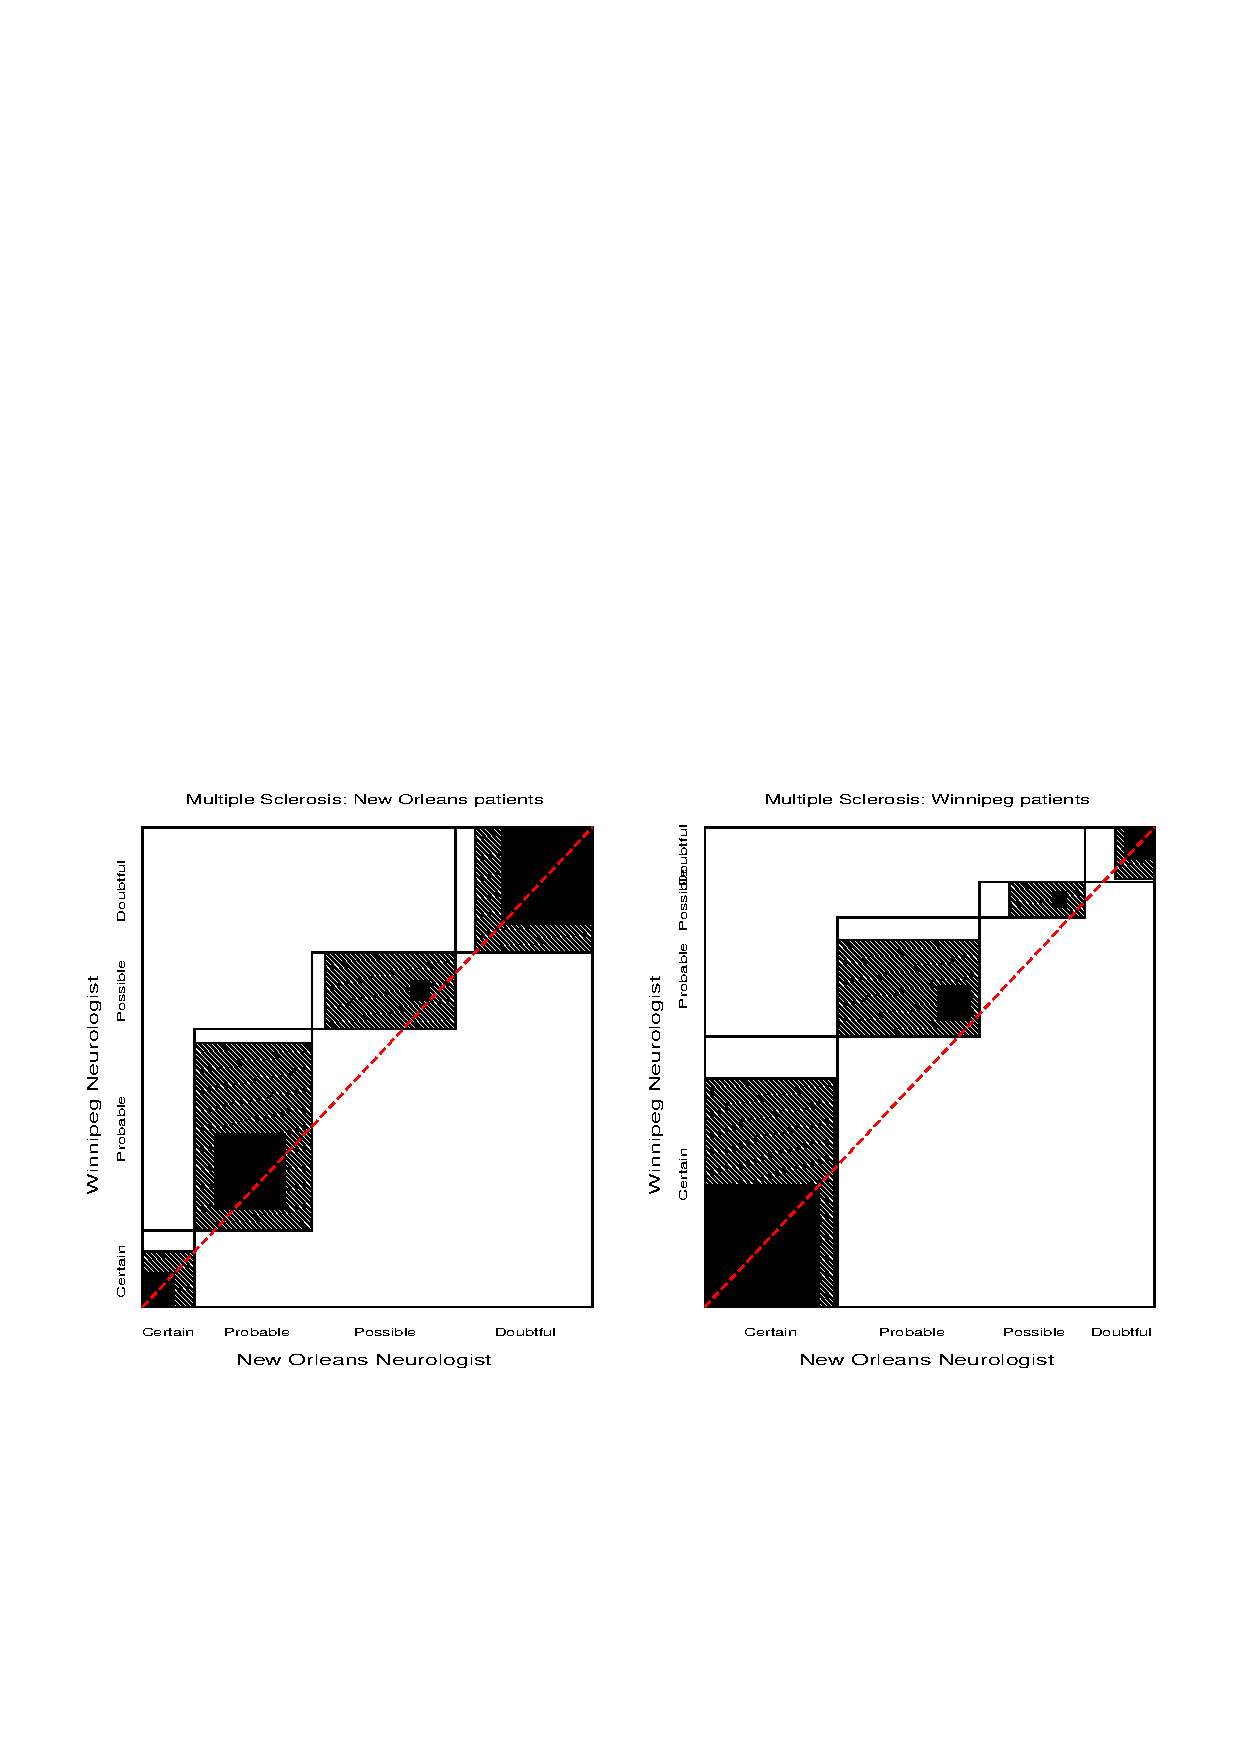
\includegraphics[width=.9\textwidth,clip]{fig/agree2}
 \end{center}
 \item Winnipeg neurologist tends to use more severe categories
  \end{itemize*}
\end{frame}

\begin{frame}[fragile]
  \frametitle{Testing marginal homogeneity}
  \begin{itemize}
	\item  Test marginal homogeneity using \PROC{CATMOD}
      \begin{itemize*}
	  \item Two tests available:
    	\begin{itemize*}
		\item Equal marginal frequencies: \texttt{RESPONSE marginals;} statement
		\item Equal mean scores: \texttt{RESPONSE means;} statement
		\end{itemize*}
      \end{itemize*}
  \end{itemize}
\begin{Input}[fontsize=\footnotesize,label=\fbox{\texttt{agreemar.sas} $\cdots$},baselinestretch=0.8]
title 'Classification of Multiple Sclerosis: Marginal Homogeneity';
proc format;
   value diagnos 1='Certain ' 2='Probable'  3='Possible'  4='Doubtful';

data ms;
 format win_diag no_diag diagnos.;
   do win_diag = 1 to 4;
   do no_diag  = 1 to 4;
      input count @@;
      if count=0 then count=1e-10;  \sascomment{/* avoid structural zeros */}
      output;
      end; end;
datalines;
   5     3     0      0
   3    11     4      0
   2    13     3      4
   1     2     4     14
;
\end{Input}
\end{frame}

\begin{frame}[fragile]
  \frametitle{Testing marginal homogeneity}
\begin{Input}[fontsize=\footnotesize,label=\fbox{$\cdots$ \texttt{agreemar.sas} $\cdots$},baselinestretch=0.8,firstnumber=20]
title2 'Testing equal marginal proportions';
proc catmod data=ms;
   weight count;
   \sasemph{response marginals;}
   model win_diag * no_diag = _response_ / oneway;
   repeated neuro 2 / _response_= neuro;
\end{Input}
Output:
\begin{Output}[gobble=5,baselinestretch=0.9]
                 Testing equal marginal proportions
                        Analysis of Variance
 
            Source         DF   Chi-Square    Pr > ChiSq
            --------------------------------------------
            Intercept       3       222.62        <.0001
            \sasemph{Neuro           3        10.54        0.0145}

            Residual        0          .           .    
\end{Output}
$\Rightarrow$ marginal proportions differ (test of \texttt{neuro})

\end{frame}

\begin{frame}[fragile]
  \frametitle{Testing marginal homogeneity}
Test of mean scores is more powerful for ordered categories:
\begin{Input}[fontsize=\footnotesize,label=\fbox{$\cdots$ \texttt{agreemar.sas}},baselinestretch=0.8,firstnumber=26]
title2 'Testing equal means';
proc catmod data=ms;
   weight count;
   \sasemph{response means;}
   model win_diag * no_diag = _response_ / oneway;
   repeated neuro 2 / _response_= neuro;
\end{Input}
Output:
\begin{Output}[gobble=5,baselinestretch=0.9]
                        Testing equal means
                        Analysis of Variance
 
            Source         DF   Chi-Square    Pr > ChiSq
            --------------------------------------------
            Intercept       1       570.61        <.0001
            \sasemph{Neuro           1         7.97        0.0048}

            Residual        0          .           .    
\end{Output}
$\Rightarrow$ test of \texttt{neuro}, on 1 df (linear) more highly significant

\end{frame}

\endinput

% slide template
\begin{frame}
  \frametitle{}
  \begin{itemize}
	\item{\large\bfseries }
      \begin{itemize*}
	  \item 
    	\begin{itemize*}
		\item 
		\item 
		\end{itemize*}
	  \item 
	  \end{itemize*}
	\item{\large\bfseries }
	\item{\large\bfseries }
  \end{itemize}
\end{frame}

